\documentclass[11pt]{article}
\usepackage[margin=1in,headheight=15pt]{geometry}
\usepackage[T1]{fontenc}\usepackage[utf8]{inputenc}\usepackage{lmodern}
\usepackage[scaled=.95]{helvet}\renewcommand{\familydefault}{\sfdefault}
\usepackage[expansion=false]{microtype}
\usepackage{amsmath,amssymb,amsthm,booktabs,tabularx,longtable,graphicx,enumitem,titlesec,fancyhdr,xcolor,tikz,xurl}
\usetikzlibrary{arrows.meta,positioning,calc}
\usepackage[numbers,sort&compress]{natbib}
\usepackage[colorlinks=true,linkcolor=Ink,citecolor=Blue,urlcolor=Blue]{hyperref}
\definecolor{Ink}{HTML}{101B23}\definecolor{Blue}{HTML}{4E758E}\definecolor{Amber}{HTML}{B18A50}\definecolor{Champagne}{HTML}{E4BD83}\definecolor{Pale}{HTML}{EDF1F3}\definecolor{Muted}{HTML}{647683}
\urlstyle{same}
\color{Ink}\hypersetup{pdftitle={Hierarchical Abstractions as a Basis for Ontology Graphs},pdfauthor={Out of Distribution Labs},pdfsubject={Theoretical foundations for software-engineering micro-agents}}
\setlength{\emergencystretch}{2em}\setlength{\parindent}{0pt}\setlength{\parskip}{7pt}
\setlist{itemsep=3pt,topsep=4pt,leftmargin=*}
\titleformat{\section}{\Large\bfseries\color{Ink}}{\textcolor{Amber}{\thesection}}{.7em}{}
\titleformat{\subsection}{\large\bfseries}{\thesubsection}{.7em}{}
\pagestyle{fancy}\fancyhf{}\fancyhead[L]{\small Out \textcolor{Amber}{of} Distribution Labs}\fancyhead[R]{\small\color{Muted}Research / 01}\fancyfoot[L]{\scriptsize\color{Muted}Hierarchical abstractions / October 2026}\fancyfoot[R]{\small\thepage}\renewcommand{\headrulewidth}{.3pt}
\newtheorem{proposition}{Proposition}\newtheorem{definition}{Definition}
\newcommand{\powerset}{\mathcal{P}}\newcommand{\ctx}{\mathsf{ctx}}\newcommand{\llbracket}{[\![}\newcommand{\rrbracket}{]\!]}
\begin{document}
\begin{titlepage}
\begin{tikzpicture}[remember picture,overlay]
\fill[Ink] (current page.north west) rectangle ($(current page.north east)+(0,-10cm)$);
\foreach \x in {0,...,19}{\foreach \y in {0,...,6}{\pgfmathsetmacro{\yy}{.22*\y+.07*sin(\x*21+\y*17)}\fill[Blue!65] ($(current page.north west)+(10+.24*\x,-5-\yy)$) circle (.35pt);}}
\foreach \x/\y in {11.3/-5.4,12.7/-6.2,14.2/-5.7}{\fill[Champagne] ($(current page.north west)+(\x,\y)$) circle (1.2pt);}
\end{tikzpicture}
\vspace*{.1cm}
{\color{white}\Large Out \textcolor{Champagne}{of} Distribution\\Labs\par}
\vspace{.8cm}
{\color{white}\fontsize{29}{34}\selectfont Hierarchical abstractions\\as a basis for\\ontology graphs\par}
\vspace{.4cm}
{\color{Champagne}\normalsize Theoretical foundations for software-engineering micro-agents\par}
\vspace{2.2cm}
{\color{Muted}\small WHITE PAPER / RESEARCH 01 / VERSION 1.0\par}
\vspace{.6cm}
{\Large Out of Distribution Labs\par}
October 7, 2026\par
\vspace{.9cm}
\textbf{Thesis.} A shared graph becomes reasoning infrastructure when abstraction is a declared preservation relationship, evidence remains recoverable, and distributed contributions obey explicit admission rules.\par
\vspace{.25cm}
\textbf{Status.} Theoretical synthesis and proposed architecture, supported by reproducible finite checks and a routing simulation. No production deployment, hundred-agent language-model experiment, or new general mathematical theorem is claimed.\par
\vfill
{\small\url{https://outofdistributionlabs.github.io/}\par
\href{https://outofdistributionlabs.github.io/research/hierarchical-abstractions/progress.html}{Research process, literature map, evaluation and project history}\par}
\end{titlepage}

\begin{abstract}
Hundreds of specialized software-engineering agents need a common way to refer to code, requirements, contracts, behavior and evidence. Messages and embedding neighborhoods do not by themselves supply that common semantics. This paper examines hierarchical abstraction as a foundation for ontology graphs, distinguishing semantic abstraction, ontological classification, retrieval organization and execution coordination. Drawing on abstract interpretation, concept lattices, behavioral subtyping, ontology modularity and distributed-state theory, we define contextual abstraction domains and task-relative sufficiency. Elementary propositions establish composition conditions, distinctions that a sufficient abstraction must retain, and a restricted condition for safe parallel vocabulary extension. Counterexamples show why lossy summaries cannot justify universal software claims and why convergent record merging can create an inconsistent ontology. We propose a typed, polyhierarchical graph with revision-scoped claims, abstraction certificates and a controlled admission projection. A reproducible simulation at 100, 300 and 1,000 logical workers illustrates structural routing consequences: a complete multi-view hierarchy matches a complete flat index, missing cross-module membership reduces recall, and coverage-aware fallback increases candidate cost. The framework treats hierarchy as a semantic interface with obligations, not a guarantee that more agents produce better software.
\end{abstract}
\section*{Reader's guide and claim status}
This paper prioritizes theoretical foundations for software engineering. Definitions, propositions and counterexamples are primary; the architecture and simulation are supporting consequences. Propositions follow from explicit assumptions and are not claimed as mathematically novel. The architecture is a proposal. Prior empirical findings retain their original scopes. All measured values concern our synthetic model, not language-model execution. The source register records access depth and versions; the project page links reproducible artifacts.
\tableofcontents\clearpage

\section{The problem: shared meaning at agent scale}
A repository contains multiple structures: files and packages, type hierarchies, call graphs, data flow, runtime dependencies, requirements and change histories. None is a complete description of the others. A function can belong to one package, implement a security-sensitive operation, and participate in several deployment workflows. A module summary may erase precisely the behavior another worker needs to verify.

Distributed specialization increases the pressure on shared meaning. A parser identifies symbols, a contract worker describes preconditions, a security worker follows effects, a test worker constructs witnesses, a patch worker changes code, and a reviewer checks evidence. Their outputs must refer to compatible revisions and vocabulary while retaining different authority and scope. Sharing a vector store does not prevent evidence about one environment from being used as a fact about another.

We use \emph{micro-agent} to mean a bounded worker with a declared role, tools, readable vocabulary and admissible effects. It may be a language-model process, deterministic analyzer, or human-assisted worker. Hundreds of registered workers need not mean hundreds of concurrent model calls or separate models. A large registry can supply a small task-specific cohort.

The central question is semantic: \emph{what must an abstraction preserve so another worker can reason through it?} Efficiency is a separate question. We propose that an ontology graph should expose preservation, grounding and context, with retrieval and scheduling attached through separate interfaces. The graph does not replace compiler semantics, testing or execution control.

\section{Research method and intellectual foundations}
\subsection{Structured narrative review}
We reviewed 22 primary-source records with a cutoff of October 7, 2026. Search families covered abstraction, concept lattices, ontology classification and modularity, software specification, graph retrieval, multi-agent coordination and distributed convergence. Inclusion required a directly relevant mechanism or formal distinction. We preferred original papers, author/publisher records, conference proceedings and normative W3C specifications; exact queries and access notes are published.

This is not an exhaustive systematic review. Several foundational records were inspected at author-summary, abstract or bibliographic level rather than read in full: abstract interpretation's author summary, the concept-analysis book, Parnas, Contract Net, the blackboard overview and SWE-bench. Hoare's scanned PDF yielded no usable local text, so its cited role is limited to the inspected primary-source passage. Full-text readings included behavioral subtyping, OntoClean's revised chapter, ontology modularity, the CRDT report, GraphRAG, HippoRAG, AutoGen, multi-agent failure analysis, agent scaling and SWE-agent. Adjacent source-code knowledge graphs and MDP abstraction were screened but are not relied on for propositions.

\subsection{Abstraction and software specification}
Abstract interpretation connects simplified representations with concrete program semantics, allowing imprecision while preserving soundness \citep{cousot1977}. Formal concept analysis orders closed extent--intent pairs induced by an object--attribute incidence relation \citep{ganter1999}. The first concerns interpretation and preservation; the second concerns structure induced by declared attributes. Neither makes an arbitrary generated summary a proof.

Parnas distinguishes criteria for decomposing a system rather than treating one convenient decomposition as inevitable \citep{parnas1972}. Behavioral subtyping constrains substitution through specifications, invariants and relevant histories \citep{liskov1994}. Hoare-style pre/postcondition reasoning makes program obligations explicit \citep{hoare1969}. These foundations suggest question-relative representations and explicit contracts, not a universal tree of code concepts.

\subsection{Ontologies, evidence and distributed state}
OntoClean uses metaproperties including identity, rigidity and unity to analyze taxonomic choices \citep{ontoclean2009}. Ontology modularity formalizes safe reuse through conservative extension and supplies locality-based sufficient mechanisms; general problems can be undecidable in expressive settings \citep{modularity2008}. OWL 2 profiles define different reasoning fragments, and Direct Semantics defines logical interpretation \citep{owl2012,semantics2012}.

SKOS supplies knowledge-organization relations, SHACL validates selected graph constraints, and PROV-O represents derivation and attribution \citep{skos2009,shacl2017,prov2013}. These are different obligations. CRDT theory supplies convergence conditions for suitable replicated state \citep{crdt2011}; convergence does not certify the logical consistency of the accumulated statements.

\subsection{Retrieval and agent systems}
GraphRAG uses hierarchical community summaries for global query-focused summarization \citep{graphrag2024}. HippoRAG integrates knowledge graphs and Personalized PageRank for evidence retrieval \citep{hipporag2024}. Topical membership and relevance scores are not certified class inclusion or truth.

Contract Net separates task announcement, bidding and award, while blackboard systems coordinate specialized knowledge sources through shared state \citep{smith1980,nii1986}. AutoGen supplies programmable conversation patterns \citep{autogen2023}. Multi-agent failure analysis distinguishes specification/design, alignment, verification and termination failures \citep{mast2025}; scaling comparisons show dependence on task and architecture, not uniform gains from adding workers \citep{scaling2025}. None establishes hundred-agent behavior for our proposal.

SWE-agent studies interfaces for repository navigation, editing and testing; SWE-bench supplies executable repository-level issue tasks \citep{sweagent2024,swebench2024}. They inform a future evaluation plan, rather than validate the ontology architecture here.

\subsection{The synthesis gap}
These mechanisms answer different questions: how to simplify semantics, organize concepts, retrieve evidence, allocate tasks and transport records. Our contribution is a proposed interface between them, not a claim that they have never been combined. An abstraction should expose preservation assumptions, a retrieved summary should expose evidence, and an accepted assertion should expose admission scope. Whether this combination improves software outcomes remains untested.

\section{Four structures, four meanings}
\begin{table}[ht]\small\centering
\begin{tabularx}{\linewidth}{@{}lXX@{}}\toprule
Structure & Relationship represented & What it does not certify \\\midrule
Semantic abstraction & Simpler representation with preserved properties & Correctness of unspecified compression \\
Ontology & Classes, instances, predicates and axioms & Behavioral substitution from names \\
Retrieval organization & Communities, summaries and relevance & Logical implication or truth \\
Coordination & Dependencies, capabilities and effects & Correctness of worker conclusions \\\bottomrule
\end{tabularx}\caption{One graph can store all four structures, but its edge types and inference rules must remain distinct.}\end{table}

A payment function is \emph{part of} a package, \emph{calls} a retry utility, and may have a contract that \emph{requires} an idempotency key. A tool report \emph{supports} a behavior claim; a module summary \emph{describes} related records; a task is \emph{assigned to} a patch worker. Replacing these relations by a generic parent edge destroys the conditions under which an inference is allowed.

Hierarchy therefore means a family of ordered views. A taxonomic view may be a DAG after equivalent classes are collapsed. Containment can be a tree or DAG. Call and dependency graphs can be cyclic. Coordination can have feedback even if one scheduled task run is acyclic. The representation must declare these choices rather than import assumptions from a visualization.

\section{Contextual abstraction domains}
\subsection{Concrete worlds and precision}
Fix $c=(r,e,v)$: repository revision, environment and specification version. Let $X_c$ denote admissible concrete software states or traces. A concrete knowledge state is $S\in C_c=\powerset(X_c)$ ordered by inclusion. More possible worlds means less precision. This is a semantic model, not a claim that all program executions are enumerable.

Let $(A_c,\sqsubseteq)$ be an abstract ordered domain with monotone abstraction and concretization maps $\alpha:C_c\to A_c$, $\gamma:A_c\to C_c$. In the standard adjunction setting,
\begin{equation}
\alpha(S)\sqsubseteq a\ \Longleftrightarrow\ S\subseteq\gamma(a).
\label{eq:adjunction}
\end{equation}
Consequently $S\subseteq\gamma(\alpha(S))$. The abstraction may include spurious possibilities but must not exclude an actual one. Completeness and computability are separate. This construction derives from established abstraction theory \citep{cousot1977}; applying it to a graph requires real interpretation maps.

For integer possibilities $S=\{2,4\}$, an interval abstraction gives $[2,4]$. It also permits 3, but does not say 3 was observed. Likewise, ``may acquire a lock'' does not mean ``always acquires a lock.'' Workers need the modality of a representation, not merely its label.

For a concrete transformer $F:C_c\to C_c$, a sound abstract transformer $F^\#:A_c\to A_c$ satisfies
\begin{equation}
F(\gamma(a))\subseteq\gamma(F^\#(a))\quad\text{for all }a.
\end{equation}
A concise LLM explanation has no such guarantee by virtue of its fluency. It can be a candidate view or a retrieval aid until its obligations are checked.

\subsection{Composition has explicit premises}
\begin{proposition}[Composition of registered abstractions]
If ordered domains $A_0,A_1,A_2$ have Galois connections $(\alpha_{01},\gamma_{10})$ and $(\alpha_{12},\gamma_{21})$, their composed maps also form a Galois connection.
\end{proposition}
\begin{proof}
For $x\in A_0,z\in A_2$,
\begin{align*}
\alpha_{12}(\alpha_{01}(x))\sqsubseteq_2 z
&\Longleftrightarrow\alpha_{01}(x)\sqsubseteq_1\gamma_{21}(z)\\
&\Longleftrightarrow x\sqsubseteq_0\gamma_{10}(\gamma_{21}(z)).
\end{align*}
These are precisely the adjunction conditions for the composite.
\end{proof}
This elementary result licenses compatible, registered paths. It does not prove code $\to$ module $\to$ service $\to$ business goal is a sound chain. A topical summary, a class relation and a behavior projection need not share domains, context or preservation properties.

\subsection{Universal properties and spurious counterexamples}
Let $\llbracket\varphi\rrbracket_c$ be the concrete worlds satisfying $\varphi$. If $S\subseteq\gamma(a)$ and $\gamma(a)\subseteq\llbracket\varphi\rrbracket_c$, then $S\subseteq\llbracket\varphi\rrbracket_c$ by transitivity. A universal property proved for all concretizations of a sound abstraction applies to the actual represented possibilities.

The reverse fails: a coarse abstraction can introduce a spurious violating world even when all actual worlds satisfy the property. A violation of the coarse model calls for a concrete witness or refinement, not an automatic bug report. Conversely, favorable observations do not prove a universal premise without a coverage argument. A passing finite test suite and a sound analysis carry different guarantees.

\section{Task-relative sufficiency and polyhierarchy}
\begin{definition}[Question equivalence and sufficiency]
For Boolean predicates $Q$ on $X_c$, define $x\sim_Q y$ when $q(x)=q(y)$ for all $q\in Q$. A map $h:X_c\to Z$ is $Q$-sufficient when every $q$ factors through $h$: $q=\bar q\circ h$ for some $\bar q:Z\to\{0,1\}$.
\end{definition}
\begin{proposition}[Necessary separation]
If some $q\in Q$ distinguishes $x$ from $y$, every $Q$-sufficient map distinguishes them.
\end{proposition}
\begin{proof}
If $h(x)=h(y)$, then $\bar q(h(x))=\bar q(h(y))$, contradicting $q(x)\ne q(y)$.
\end{proof}
For finite $X_c$, the quotient $X_c/{\sim_Q}$ is a sufficient partition; every sufficient partition refines it. This gives a lower bound on the distinctions the question family demands. It neither makes equivalence decidable for arbitrary program behavior nor provides an automatic way to infer all relevant questions from a request.

\subsection{A cache counterexample}
Two cache implementations have identical sequential outputs. One invalidates atomically; the other permits a concurrent reader to observe stale data after invalidation. A summary retaining only sequential input/output behavior maps them to the same representation. It is insufficient for ``can a stale read occur after invalidation?'' It may remain sufficient for a recorded sequential test question.

API, effect, security and deployment views should therefore coexist. An interface-discovery view can be inadequate for concurrency verification. Refinement can preserve one necessary distinction without expanding every summary into the entire codebase. The graph should retain which question family a view serves and the witness that caused a split.

\subsection{Concept lattices do not certify incidence}
Formal concept analysis begins with $(O,M,I)$: objects, attributes and incidence. Derivation operators yield closed extent--intent pairs ordered by extent inclusion \citep{ganter1999}. This supports overlapping classification without requiring a tree. It does not establish the truth of $I$.

In software, ``passed retry test'' and ``may access credentials'' have different modalities. Measured attributes need revision and environment scope; possible effects must not be turned into recorded runtime occurrences. A lattice built from mistaken incidence is orderly but mistaken. We use it as organization of declared information, with evidence admission treated separately.

\section{A typed graph and its accepted interpretation}
\subsection{Candidate records versus logical content}
Let $G_r=(V,E,\tau,\kappa,P)$ be a snapshot: nodes and edges, sorts $\tau$, contexts $\kappa$, and provenance links $P$. Let $T_r$ be a separate set of admitted axioms. Adding a candidate claim record to $V$ does not automatically add its asserted formula to $T_r$.

Useful sorts include Artifact, Concept, Requirement, Contract, Observation, Claim, Task, Capability and Context. An ontology class is not a source-code object with the same printed name. A test run is an observation, not a proof by default. Predicate signatures expose these distinctions operationally.

\begin{table}[ht]\small\centering
\begin{tabularx}{\linewidth}{@{}lXX@{}}\toprule
Predicate & Intended relation & Inference boundary \\\midrule
subClassOf & Logical class inclusion & Compatible interpretation and context \\
partOf & Composition or containment & Does not imply subclass membership \\
calls / dependsOn & Dependency & Does not transfer all properties \\
summarizes & Grounded view & No entailment without preservation conditions \\
supports / derivedFrom & Evidence and provenance & No automatic truth or independence \\
assignedTo & Allocation & No verification guarantee \\\bottomrule
\end{tabularx}\caption{Illustrative relation contracts; an implementation must provide actual schemas and semantics.}\end{table}

\subsection{Context, identity and multiple parents}
A function can be part of a payment module, meet an idempotency contract, and participate in a sensitive-effect view. These are different paths. For this application we propose acyclic taxonomic views after declared equivalences are collapsed. This is an application invariant, not a universal constraint on OWL or SKOS. Other graph relations can remain cyclic.

Use revision-qualified identifiers, source hashes and explicit rename/move lineage. Matching paths do not prove identity: a symbol can be deleted and recreated at the same location. A move can preserve identity while invalidating location-based evidence. Identity mappings themselves need provenance and review.

OntoClean's stable-kind versus contextual-role distinction informs this design \citep{ontoclean2009}. ``Assigned reviewer'' is a role, not necessarily a permanent agent superclass. ``Currently failing test'' refers to an observation under a revision and environment, not an intrinsic type of a file.

\subsection{An abstraction certificate}
A promoted abstraction relationship should expose: source/target sorts; concrete context; interpretation maps or an explicitly weaker relation; preserved question family or property fragment; evidence witnesses and proof obligations; validation method; source hashes; and invalidation conditions. A missing obligation does not forbid storing the view: it changes its status to hypothesis or retrieval aid.

This certificate is a proposed interface, not an assertion that all obligations are automatically decidable. Restricted analyses can discharge some formally; informal requirements may require review. ``Proof-backed,'' ``validated on selected tests'' and ``unverified summary'' should remain distinguishable in every downstream use.

\subsection{Four independent checks}
Class inclusion $A\subseteq B$ transfers universal properties of $B$ to $A$ under one interpretation. It does not transfer an arbitrary existential witness in $B$ into $A$, and it does not prove implementation substitutability. Behavioral substitution concerns preconditions, postconditions, invariants and relevant history constraints \citep{liskov1994}.

OWL open-world entailment and SHACL validation must remain separate \citep{semantics2012,shacl2017}. A missing required field can fail a selected shape without entailing that a real-world relation is false. SKOS broader is not itself declared transitive, and broaderTransitive is distinct \citep{skos2009}; a knowledge-organization edge must not silently become a subclass axiom.

PROV records origin and derivation \citep{prov2013}, not truth, calibrated confidence or source independence. Ten summaries derived from one test remain one underlying observation. Authorization is a fourth concern: semantic relevance to a file does not grant a worker permission to edit it.

\section{Safe evolution and distributed admission}
\subsection{Convergence can preserve a contradiction}
CRDT convergence applies under declared algebraic and delivery assumptions \citep{crdt2011}. Consider $T_0$ declaring $A$ and $B$ disjoint, with proposals $\Delta_1=\{A(a)\}$ and $\Delta_2=\{B(a)\}$. Each extension of $T_0$ has a model, but $T_0\cup\Delta_1\cup\Delta_2$ does not. Claim records can converge perfectly while their admitted interpretation becomes inconsistent. Record convergence and semantic admission are independent obligations.

We propose an append-only candidate log and a controlled accepted projection. Identity merges, competing contracts and schema edits are non-monotone choices requiring checks or serialized governance. Retractions should preserve supersession/tombstone history. A deterministic admission pipeline can check authorization, signatures, shapes, revision dependencies, selected logical consistency conditions and evidence policy. It should record which criteria passed rather than flatten them into ``verified.''

\subsection{Conservative extension and parallel vocabulary}
For signature $\Sigma$, a deductive conservative extension preserves old $\Sigma$ entailments:
\begin{equation}
\forall\varphi\text{ over }\Sigma,\quad T'\models\varphi\ \Longleftrightarrow\ T\models\varphi.
\end{equation}
A model-conservative extension is stronger: every model of $T$ can be expanded, on the same domain and with old symbols unchanged, to a model of $T'$. These notions underlie ontology modularity \citep{modularity2008}.

\begin{proposition}[Independent private vocabulary extension]
Let $T$ use signature $\Sigma$. For $i=1,2$, let $T_i=T\cup\Delta_i$ be model-conservative over $T$ using private signatures $\Sigma_i$ disjoint from $\Sigma$ and from each other. Suppose $\Delta_i$ mentions only $\Sigma\cup\Sigma_i$. Then $T\cup\Delta_1\cup\Delta_2$ is model-conservative over $T$.
\end{proposition}
\begin{proof}
Take a model $M$ of $T$. Each premise supplies an expansion $M_i$ on the same domain, preserving $M$ on $\Sigma$. Interpret the private symbols in $\Sigma_1$ as in $M_1$ and those in $\Sigma_2$ as in $M_2$. Disjointness makes this combined interpretation well-defined. Every axiom of $\Delta_i$ sees exactly its interpretation from $M_i$, so both sets hold. The combination expands the arbitrary model $M$ of $T$.
\end{proof}
This elementary sufficient condition explains a limited form of parallel semantic work. It does not license overlapping contract edits, shared identity changes or arbitrary claim additions. The disjointness counterexample fails the conservativity premises. Ordinary code ownership does not establish them either.

General conservativity checking can be undecidable in expressive ontology settings. Locality extraction provides useful sufficient mechanisms, but a nearby graph neighborhood is not automatically a logical module \citep{modularity2008}. Restricted profiles, extracted modules and finite regression query suites are practical alternatives. Passing a finite suite certifies that suite, not full conservativity. Intentional corrections may legitimately change old entailments; those changes should be explicit and communicated.

\section{Execution contracts and software workflows}
Represent a worker interface as
\begin{equation}
a=(\rho,\Sigma_R,W,\mathcal U,\mathit{Pre},\mathit{Out},\mathit{Verify},B),
\end{equation}
where the entries are role, readable signature, write scope, tools, preconditions, output shapes, verification policy and budget. A worker reads an immutable snapshot, selects a relevant view, expands to grounded artifacts, performs a bounded action and proposes a delta with evidence.

Read dependencies matter as much as edited files. Two workers can edit different files while one depends on a contract the other changes. Revision checks should cover the relevant dependency closure or mark the result stale. A graph records these dependencies; scheduling and execution isolation enforce them.

\begin{figure}[ht]\centering
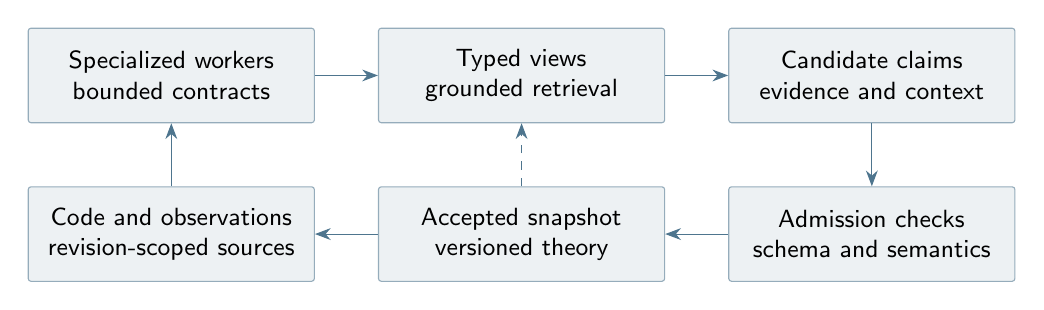
\begin{tikzpicture}[node distance=8mm and 8mm,box/.style={draw=Blue!60,rounded corners=1pt,fill=Pale,align=center,font=\small,minimum height=12mm,text width=34mm},arr/.style={-{Stealth[length=2mm]},draw=Blue}]
\node[box] (a) {Specialized workers\\bounded contracts};\node[box,right=of a] (b) {Typed views\\grounded retrieval};\node[box,right=of b] (c) {Candidate claims\\evidence and context};\node[box,below=of c] (d) {Admission checks\\schema and semantics};\node[box,left=of d] (e) {Accepted snapshot\\versioned theory};\node[box,left=of e] (f) {Code and observations\\revision-scoped sources};
\draw[arr] (a)--(b);\draw[arr] (b)--(c);\draw[arr] (c)--(d);\draw[arr] (d)--(e);\draw[arr] (e)--(f);\draw[arr] (f)--(a);\draw[arr,dashed] (e)--(b);
\end{tikzpicture}\caption{Proposed interfaces. Candidate storage is not semantic acceptance. Dashed feedback exposes accepted snapshots to retrieval.}\end{figure}

For safe concurrent payment retries, a requirements worker records the intended property and ambiguities. Parser/effect workers ground symbols and possible side effects. A contract worker identifies idempotency obligations. A counterexample worker seeks violating interleavings. A patch worker proposes a revision; verification workers run selected analyses and tests. Admission checks the evidence and policy before producing a new accepted snapshot. Security and integration concerns may cut across package ancestry; the workflow requires a disagreement path, not only a success path.

Hundreds of workers can share vocabulary while only a bounded cohort executes a task. Their role and relevance do not grant identical write authority. Textual consensus is not a proof, and all tools may share the same mistaken assumptions. Failure patterns reported in multi-agent systems motivate explicit verification and termination policies, not an assumption that a graph automatically removes them \citep{mast2025}.

\subsection{A worked admission trace}
Suppose revision $r_0$ has a function \textsf{charge(key, amount)} and a requirement that concurrent retries must not create duplicate ledger entries. A module summary says ``the payment service is idempotent.'' That sentence is only a candidate claim until its modality and evidence are resolved.

The parser grounds the function and ledger operation. A unit-test worker reports two sequential retries yielding one entry in environment $e_0$. Its claim is an observation about those executions. A contract worker proposes the stronger predicate that all admitted concurrent traces contain at most one entry for a key. An effect worker finds a check-then-write path; a counterexample worker constructs two overlapping executions that both see an absent key. This witness separates traces the original summary identified.

The accepted projection may admit the unit-test observation while refusing the universal contract. It retains the contradiction witness and marks the old summary insufficient for the concurrency question. A patch worker proposes an atomic ledger insertion at $r_1$; verification runs at $(r_1,e_0,v_0)$, not silently at the old context. Passing a new stress test is still empirical evidence, while a proof about the atomic operation depends on its specified semantics and environment assumptions.

This trace explains what the hierarchy contributes: navigation from requirement to contract to grounded operations, and a location to refine a failed abstraction. It does not decide the atomicity of an external database by itself. If a later environment changes the transaction semantics, the certificate's dependency invalidates even if the source function is unchanged.

\section{Scaling and out-of-distribution refinement}
\subsection{Arithmetic bounds are not performance laws}
A complete directed all-to-all topology has $N(N-1)$ possible edges. A policy notifying at most $k$ workers creates at most $k$ deliveries per update. For balanced disjoint buckets, selecting $b$ of $B$ buckets contains approximately $Nb/B$ workers. These are counting statements with assumptions, not a theorem that ontology use makes total coordination linear.

Skew, overlapping expertise, broad requests and cross-cutting effects alter cohort size. A flat inverted index with the same memberships can select the same workers. Index maintenance, validation, replication, rework and model execution remain separate costs:
\begin{equation}
C_{\rm task}=C_{\rm route}+C_{\rm grounding}+C_{\rm workers}+C_{\rm validation}+C_{\rm rework}.
\end{equation}
Graph construction/maintenance must additionally be measured or amortized under a stated workload. Agent-scaling evidence motivates testing task--architecture alignment \citep{scaling2025}, not claiming a universal savings factor.

\subsection{OOD as a failure of an interface assumption}
Software OOD conditions include unfamiliar APIs, unrepresented effects, missing schema relations, changed dependencies, incompatible environments, stale evidence and counterexamples to a contract. A novel embedding does not calibrate the chance an inference is wrong.

Separate four flags: outside-schema evidence; unsupported preservation step; insufficient evidence coverage; and logical conflict. A flag should identify an affected view/claim and trigger grounding, refinement, abstention or review. It should not automatically induce a global schema change.

A refinement procedure retains the witness, locates the representation that merged distinguishable cases, proposes a local split or relation, reruns affected checks and records supersession. A concurrency witness may require a trace/effect view, not a source-code superclass. Broadening a concept to absorb every exception can make its preserved properties vacuous.

\section{Synthetic illustration: routing and missing membership}
\subsection{Design and measurement}
Our Python simulation uses 100, 300 and 1,000 logical workers, 16 modules with four skills each, 20 seeds (0--19), and 300 generated requests per seed/condition. Each worker receives a primary module/skill label and a secondary label in another module with probability $0$, $.25$ or $.5$. Labels also define eligibility truth.

Baselines are broadcast, complete flat index, primary-only hierarchy and guarded complete multi-view hierarchy. Local queries select one module/skill. Cross-cutting queries select one skill in four modules. Coverage-gap queries select a local label while each label's coverage flag is independently false with probability $.1$; the guard then broadcasts. Coverage detection is an oracle in this model, not an implemented OOD detector.

We measure candidates, eligible-worker recall and structural index visits. Visits count selected nodes and coverage checks, not runtime latency. Candidates can be interpreted as notification counts only for a policy sending one notification per candidate. No LLM is called, patch generated or token saving measured.

\begin{table}[ht]\centering\small
\begin{tabularx}{\linewidth}{@{}XXrrr@{}}\toprule
Scenario & Strategy & Candidates & Recall & Visits \\\midrule
local & broadcast & 300.00 & 1.000 & 0.0 \\
local & flat index & 7.07 & 1.000 & 1.0 \\
local & primary hierarchy & 4.69 & 0.664 & 4.0 \\
local & guarded multiview & 7.07 & 1.000 & 5.0 \\
cross cutting & broadcast & 300.00 & 1.000 & 0.0 \\
cross cutting & flat index & 27.73 & 1.000 & 4.0 \\
cross cutting & primary hierarchy & 18.80 & 0.678 & 11.9 \\
cross cutting & guarded multiview & 27.73 & 1.000 & 15.9 \\
coverage gap & broadcast & 300.00 & 1.000 & 0.0 \\
coverage gap & flat index & 7.03 & 1.000 & 1.0 \\
coverage gap & primary hierarchy & 4.67 & 0.663 & 4.0 \\
coverage gap & guarded multiview & 38.71 & 1.000 & 5.0 \\
\bottomrule
\end{tabularx}\caption{Means at 300 workers and $.5$ secondary-membership probability, averaging 20 seed-level means. Recall excludes empty eligible sets. Full raw records, retained counts and seed standard deviations are published.}\label{tab:results}\end{table}

\subsection{Results and interpretation}
Local requests select 7.07 workers on average under both complete strategies, versus 300 under broadcast. The primary-only hierarchy selects 4.69 but retains only .664 eligible-worker recall. Cross-cutting requests select 27.73 under the complete strategies, versus 18.80 and .678 recall under primary-only membership. For coverage gaps, guarded recall stays 1.000 but candidate count rises to 38.71; the complete flat baseline selects 7.03. These are generated-label results, not measurements of software competence.

\begin{figure}[ht]\centering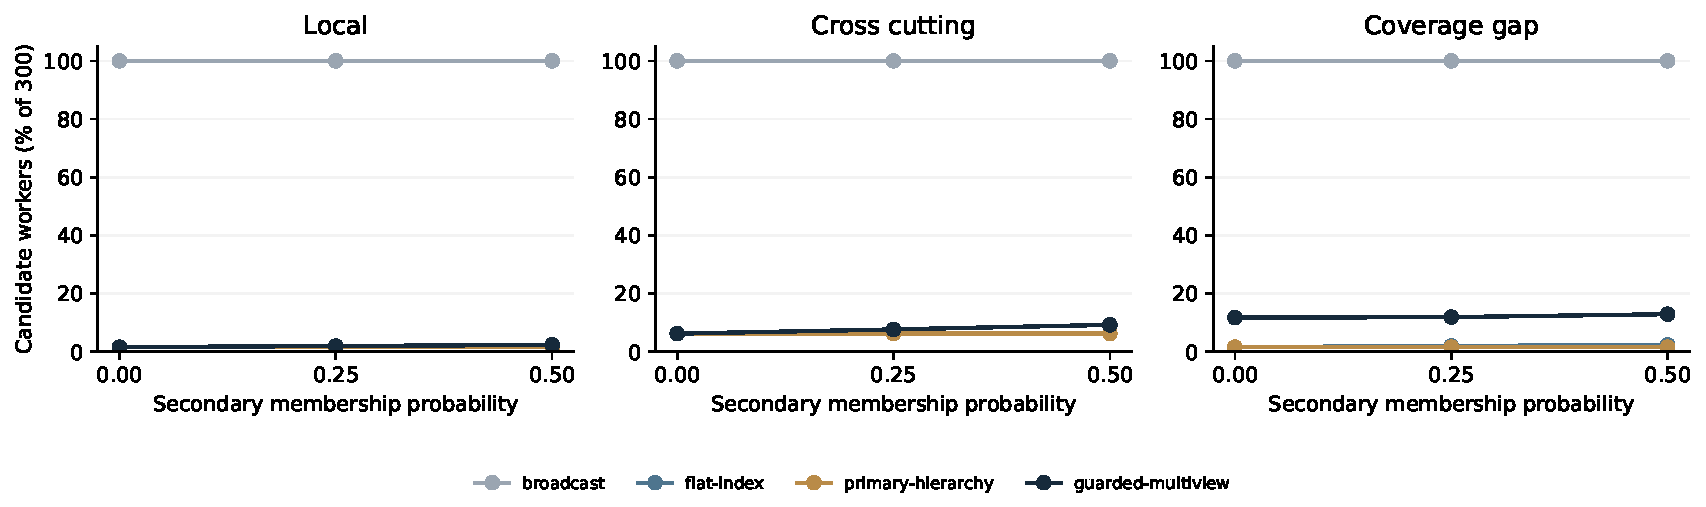
\includegraphics[width=\linewidth]{figures/routing.pdf}\caption{Candidate fractions at 300 workers. Complete flat-index and multi-view curves coincide without fallback. Broadcast is a weak routing baseline, not evidence that hierarchy outperforms an equivalent index.}\end{figure}
\begin{figure}[ht]\centering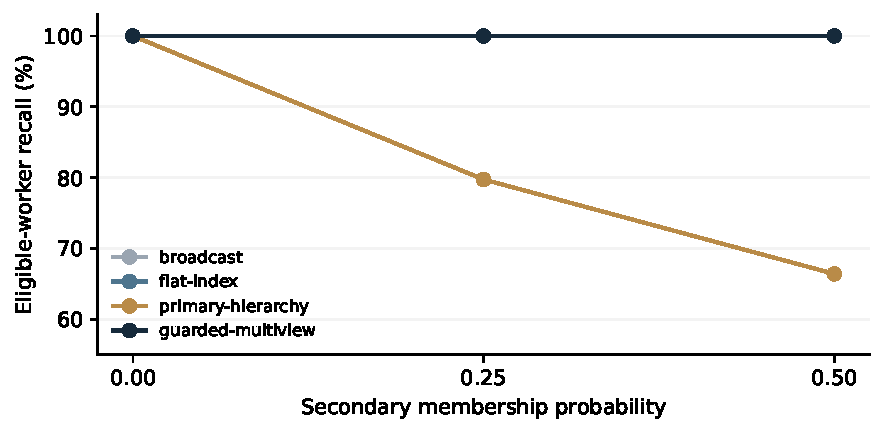
\includegraphics[width=.72\linewidth]{figures/recall.pdf}\caption{Local recall. Loss results from omitted secondary membership in the primary-only ablation. Complete strategies coincide at 100\%; this is not an intrinsic failure of every hierarchy.}\end{figure}

The simulation illustrates a distinction visible in the formal model: a smaller cohort may result from missing information rather than successful abstraction. Complete hierarchy and flat indexing produce the same candidate sets without fallback. Hierarchy's potential semantic advantage is not established by these counts.

The raw data contains 2,160 seed/strategy records. Uncertainty is sample standard deviation of seed-level means, not a confidence interval. Empty eligible sets are excluded from recall and retained counts are published; conditioning affects small-$N$ averages. Input and truth use the same generator, so complete-index recall is guaranteed by construction. Maintenance, stale state, parser errors, actual messages, contention and patch quality are outside the model. Perfect coverage detection is deliberately favorable and requires separate empirical validation.

\section{Implementation and empirical research agenda}
Start with a bounded vocabulary of artifacts, contracts, claims and contexts, deterministic symbol extraction, separate candidate/accepted projections, immutable snapshots and structured delta proposals. Use a declared reasoning fragment rather than unrestricted generated axioms. OWL profile properties constrain logical work but do not guarantee low end-to-end latency \citep{owl2012}.

A future study should compare single-agent execution, unstructured multi-agent memory, a complete flat typed index, hierarchy without certificates, and hierarchy with certificates/admission. Match models, tools, repository snapshots, evidence and task budgets. Distinguish registry size from concurrently active cohort size. A 1,000-worker registry with five active workers is not a concurrent 1,000-agent experiment.

Tasks should include bug localization, change impact, security analysis and patch generation. SWE-bench-style executable tasks offer one starting point \citep{swebench2024}; supplement test-defined success with hidden tests, static checks, domain obligations and review. Keep development tasks separate from held-out evaluation; stress unseen repositories, dependency changes and stale observations.

Measure verified outcomes, unsupported-claim rate, evidence recall, stale-read rejection, conflict detection, provenance recovery and cost per verified result. Separate wall-clock/model-call costs from graph operations. Include graph construction and update overhead. A hierarchy that improves explanation but not patch success may still have value, but it should be evaluated against that stated purpose.

Theoretical questions remain: how to infer a useful question family from requirements; which certificates admit tractable checks; how to align multiple views after code changes; and how to detect coverage gaps without equating novelty with error. An elegant ontology cannot repair incorrect concrete semantics; a useful grounded analyzer need not require a rich ontology.

\section{Limitations and conclusion}
This paper supplies a synthesis, definitions, elementary proofs, counterexamples and a proposed interface. It does not establish mathematical novelty, a complete software ontology, an implemented semantic reasoner or empirical improvement for hundreds of LLM agents. The review is source-traceable but not exhaustive; limited access to some foundational sources is disclosed. Simulation results concern generated labels, not a deployment.

The central principle is to make abstraction a declared relationship with preservation obligations. Distinct views answer distinct questions; typed relations prevent association from masquerading as entailment; revision scope prevents evidence from crossing contexts silently; and admission separates convergent storage from accepted theory. These foundations make an ontology graph a plausible semantic interface for many specialized workers. Its practical value must be tested through verified software outcomes with strong simple baselines and explicit failure cases.

\clearpage\appendix
\section{A minimal certificate interface}
\begin{table}[ht]\small\centering
\begin{tabularx}{\linewidth}{@{}lX@{}}\toprule
Field & Meaning \\\midrule
Claim identity & Immutable record distinct from its asserted formula \\
Context & Revision, environment, specification and viewpoint \\
Typed assertion & Predicate with declared source/target signature \\
Evidence status & Hypothesis, observation, checked obligation or proof-backed claim \\
Evidence lineage & Source hashes, tool run, conditions and provenance \\
Preserved questions & Property fragment or question family covered \\
Dependencies & Read symbols/certificates invalidated on change \\
Admission & Accepted, disputed, rejected or superseded, with reason \\\bottomrule
\end{tabularx}\caption{Proposed interface. Confidence scores require their own calibration method and evaluation.}\end{table}

A test report states revision, environment and tested conditions. A universal contract states proof or abstraction assumptions. A patch worker must not upgrade the former into the latter to fill a schema. This discipline can be implemented before a complex ontology is adopted.

\section{Finite checks and reproduction}
The general proofs appear in the main text. The supporting script enumerates a finite concrete domain:
\[X=\{-2,-1,0,1,2\}.\]
It checks its powerset, intervals and coarser intervals with endpoints $\{-2,0,2\}$. It checks 512 concrete--interval adjunction instances, 112 interval--coarse instances and 224 composed instances, plus the summary and merge counterexamples. These are finite sanity checks, not machine proofs for arbitrary programs.

From the project folder:
\begin{quote}\small\textsf{python evaluation/simulate.py}\\\textsf{python evaluation/check\_formal.py}\\\textsf{python evaluation/plot.py}\\\textsf{latexmk -pdf white-paper.tex}\end{quote}
Simulation/checking use Python's standard library; plots require Matplotlib. The PDF uses pdfLaTeX/BibTeX and ordinary TeX Live packages. Raw CSV, aggregate JSON, plots, notes and source records are published. Bibliographic years reflect original publication/preprint dates with pinned revisions noted in the bibliography.

\section{Reusable research process}
The shared runner \textsf{tools/research/run.py} reads project configuration, renders a static progress page, commits explicit project paths, pushes and sends ntfy. A two-minute heartbeat refreshes status while running; it does not itself perform research or independently certify progress. Completion stops it.

The six stages are protocol, literature, synthesis, evaluation, manuscript review and publication verification. The template requires scope confirmation, source/version tracking, claim-status distinctions, appropriate baselines, reproducible evidence and final artifact checks. It is a reusable process rather than a prescription for the answer.

\clearpage\begingroup\small\setlength{\bibsep}{5pt}\bibliographystyle{plainnat}\bibliography{references}\endgroup
\end{document}
